% 	HTML5 Robot User Interface Project Report: Technology Overview
% 	An ASLab Project,
% 	Developed by Daniel Peiró
% 	ETSII, UPM 2014-2015
\chapter{Technology Overview}
This chapter will give a general overview of the technologies used in the development of this project. 
This will loosely entail, for each section, a brief history, the current state of the art and how it relates 
to the project. By no means is this intended to be a comprehensive in depth look into each subject, given that 
entire books can and have been written on each of them, but should give the reader enough information to understand 
the following chapter, that details how the system is built and what it does with these technologies.
\section{HTTP}

HTTP (Hypertext Transfer Protocol) is the data communication protocol underlying in what is known today as the World
Wide Web. The idea of hypertext (a text that contains links to other texts) was first defined in the 1960s by Ted
Nelson (inspired by the Memex, a microfilm linked database envisioned by Vannevar Bush in 1945), founder of Project
Xanadu, the first attempt at an implementation of the idea. Several other implementations appeared in the following
decades (Douglas Engelbart's oN-Line System, Apple's Hypercard, Tim Berners-Lee's own ENQUIRE), but none of them
married the concept with the idea of the internet, which had been developed independently from it's origins (ARPANET
and TCP and later TCP/IP) in the late 1960s. Not until Tim Berners-Lee, a computer scientist working at CERN in 1989,
took his existing ENQUIRE hypertext database and the existing TCP/IP protocol and thought to make a network of
documents, linked between each other to form a web, that he called the ``WorldWideWeb'' or W3. To do that he needed
essentially three things: a standard language to write hypertext in, unique identifiers for each document and a
protocol to transfer these documents around the network. The first is HTML, which will be covered in the next section,
the second is the URL (Uniform Resource Locator, which won't be covered due to being only tangentially related to the
project) and the last of course is HTTP. There were other protocols that essentially achieved the same goal, most
notably Gopher, which still exists, but in the 1990s the World Wide Web became ubiquitous and synonymous with the
Internet, mainly thanks to the Mosaic Web Browser's popularity following its release in 1993. Today HTTP is the main
protocol (frequently combined with SSL/TLS to form the HTTPS protocol for enhanced security) used in the world to
communicate through the internet.\\

HTTP implements a typical Client-Server stateless pattern with a request-response communication architechture. What
stateless means is that every transaction between client and server is independent from any other. In other words,
HTTP treats every connection as a new one, given that it has no ``memory'' of any others before it. The sequence of
events that define one transaction, define the whole protocol. The basic steps that take place in one such transaction
are:
\begin{enumerate}
\item The Client opens a connection to the server (through a TCP/IP socket, typically on the standard port 80) and
sends a request, which looks something like this:
\begin{minted}[breaklines,fontsize=\footnotesize]{http}
GET / HTTP/1.1
Host: www.w3.org
Connection: keep-alive
Accept: text/html,application/xhtml+xml,application/xml;q=0.9,image/webp,*/*;q=0.8
User-Agent: Mozilla/5.0 (X11; Linux x86_64) AppleWebKit/537.36 (KHTML, like Gecko) Chrome/43.0.2357.81 Safari/537.36
Accept-Encoding: gzip, deflate, sdch
Accept-Language: es-ES,es;q=0.8,en;q=0.6
Cookie: authorstyle=no
\end{minted}
This example is taken from a Chrome Browser ``development tools'' window (accesible with Ctrl+Shift+J), when opening
the http://www.w3.org URL.\\

This simple text message is asking the server to GET (HTTP Method) the path ``/'' (the root path) with version 1.1 of
the HTTP Protocol. The rest of the text is not required (HTTP 1.1 does require the Host Header to be present), but
adds additional information to the request. The Connection ``keep-alive'' header is added to use one TCP connection
for all requests and responses, instead of opening and closing a connection on each request, to reduce overhead (this
is standard in HTTP 1.1). The Accept Header tells the server what type of content it expects (in this case it prefers
html, xhtml or xml, or with less preference represented by the q value from 0 to 1, an image, or with even less
preference, anything else). The user agent tells the server which platform is making the request, and so on.
\item The server responds (through the same TCP connection):
\begin{minted}[breaklines,fontsize=\footnotesize]{http}
HTTP/1.1 200 OK
Date: Fri, 05 Jun 2015 17:13:20 GMT
Server: Apache/2
Content-Location: Home.html
Vary: negotiate,accept
TCN: choice
Last-Modified: Fri, 05 Jun 2015 14:20:15 GMT
ETag: "a290-517c5fda505c0;89-3f26bd17a2f00"
Accept-Ranges: bytes
Content-Length: 41616
Cache-Control: max-age=600
Expires: Fri, 05 Jun 2015 17:23:20 GMT
P3P: policyref="http://www.w3.org/2014/08/p3p.xml"
Content-Type: text/html; charset=utf-8
\end{minted}
Which indicates that using HTTP version 1.1, the request was attended correctly (code 200 OK), the server is an Apache
2.0 Server, the date and time of response, the name of the resource, the content type etc.
\item The connection is closed (in this case it would remain open since the protocol is version 1.1 and keep-alive was
specified).
\item The Server waits for another request on port 80.
\item The client uses the resource served. In most cases, the client would be a web browser, that would parse the
html, and present it to the user. This would in turn force the browser to request more resources (images, css,
scripts, etc.) that are embedded in the html (see Figure 3.1).
\end{enumerate}
\begin{figure}[ht]
	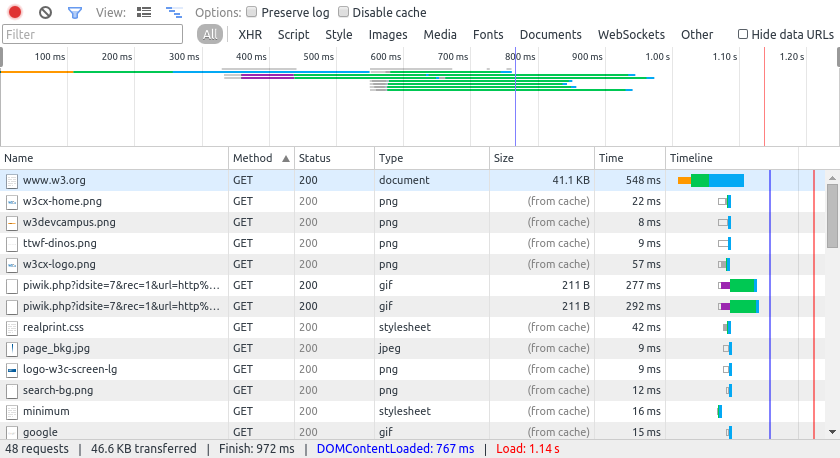
\includegraphics[width=\linewidth]{HTTP_Example}
	\caption{Google Developer Tools window showing HTTP Requests}	
\end{figure}

In the above example only the GET HTTP method is used, because the client only requests data from the server, without
sending any data itself. If the client needs to send data to the server, such as form data, or a file, it would still
initiate the connection (the server cannot make requests, only respond, another consequence of statelessness), using
the POST method. While this approach is suitable for a passive, document-based web, where interaction is limited to
jumping from document to document, the web has quickly evolved into an application-based model, where full UIs take
place in the browser space, requiring data be constantly sent back and forth between client and server, in realtime.
This project is one such application.\\

The only way to do this with standard HTTP is periodic polling, which entails large server and network loads. Some
stopgap solutions exist to minimize this overhead, most relevant of which is the Comet web application model. Comet is
based on the concept of long-polling: effectively ``hanging'' the server response until the requested data is
available, and calling another request once the data is received. This approach  still causes increased server loads
but allows some semblance of realtime data transmission. The possibility to use only one connection, as seen in the
previous example was another improvement that became standard in HTTP 1.1. With the HTTP/2 Standard (published in May
2015), the server is allowed to effectively ``push'' data to clients by queuing up more responses than received
requests. However, none of these modifications and hacks are a complete, elegant solution to the problem, given that
HTTP was never intended to be a realtime protocol.\\

That is why other technologies have taken over this new realm of interactivity, providing much more than the ``big,
virtual documentation system in the sky'' \cite{bernerslee09} envisioned by Berners-Lee more than 25 years ago. Some
of them are key parts of this project, as the following sections describe. Still, HTTP remains the initiator for all
these other technologies to function. As of today, any web page you open, no matter how complex the code served in
javascript or flash or any other plugin still begins with a simple GET request and response.
\section{HTML}
HTML (Hypertext Markup Language) is the language in which web pages are written. It was created in 1989 by Tim
Berners-Lee as part of his WorldWideWeb, a set of documents linked between each other on a network using the internet
protocol. It was initially based on SGML (Standard Generalized Markup Language) a document markup language released in
1986 as an ISO Standard (ISO 8879:1986 -- Information processing -- Text and office systems), which was itself derived
from GML (both an acronym for Generalized Markup Language and for Goldfarb, Mosher, Lorie, the last names of its
developers), developed by IBM in 1969.\\

Markup languages in general existed before digital media and still exist in paper based documentation (blue/red
annotations used by editors because litography/photography/xerography did not capture these colors, the engineering
code for editing documents red = add, blue = delete, green = comment, and many others). In general, markup is a way to
add information regarding the document's structure, presentation, state of development, comments, author, date,
copyright, etc. in a way that is distinguishable from the content of the document. For digital media, it also needs to
be machine-readable, which simply means that a computer must be able to parse this data to extract information. There
are basically two ways of doing this:
\begin{enumerate}
	\item Procedural Markup: A source text is written with instructions for a processing program (equivalent to a
  compiler) to construct the final document. A good example of this method is \TeX, the typesetting system underlying
  the \LaTeX\ macro language (which is itself a mixture of procedural and declarative markup), used to write this
  document.
	\begin{figure}[ht]
    \subfloat[Procedural Source (\LaTeX)]{{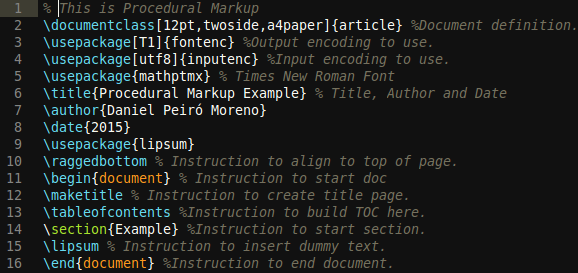
\includegraphics[width=\linewidth/2]{procedural}}}
    \subfloat[Procedural Output (PDF)]{{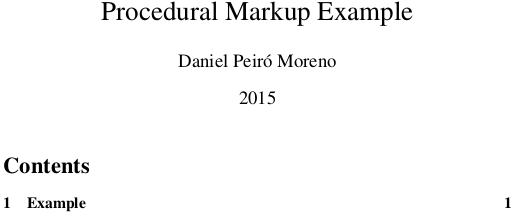
\includegraphics[width=\linewidth/2]{procedural_out}}}
    \caption{Procedural Markup Example}
	\end{figure}
	\item Declarative or Descriptive Markup: The content of the text is labeled or ``tagged'' with the markup, without
  giving any instructions on how to process these labels. HTML (especially before HTML5) and XML are clear examples of
  this method.
	\begin{figure}[ht]
    \subfloat[Declarative Input (HTML5)]{{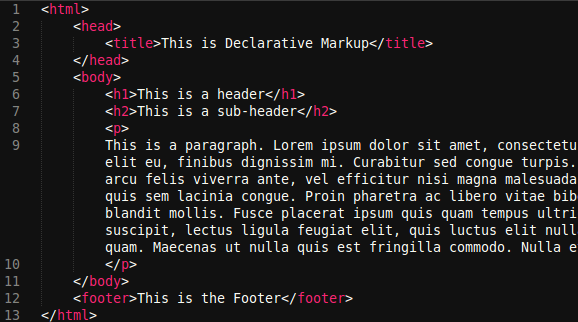
\includegraphics[width=\linewidth/2]{declarative}}}
    \subfloat[Declarative Output (Google Chrome)]{{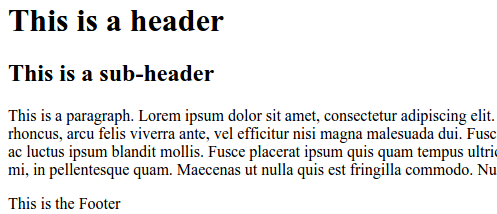
\includegraphics[width=\linewidth/2]{declarative_out}}}
    \caption{Declarative Markup Example}
	\end{figure}
\end{enumerate}
HTML and its precursor SGML are essentially declarative markup languages. The main advantage of declarative markup,
and more generally the declarative programming paradigm is the decoupling of the intended result and the processing
required to achieve it. This has been crucial for HTML to be able to evolve and adapt dinamically over decades of
technological innovation. The computers and programs used in 1989 have very little in common with those used today in
many cases. A markup language designed to be ubiquitous, read on an ever changing array of software and hardware
platforms and permanently backwards compatible, where a web page designed in 1991 is just as valid as one designed
using the last specification, has to be as procedurally oblivious as possible.\\

The basic HTML markup unit is the tag. A tag is simply a keyword surrounded by brackets. HTML tags usually come in
pairs, an opening tag and a closing tag (designated adding a forward slash after the first bracket), that give markup
information on the enclosed content:
\begin{figure}[ht]
\begin{minted}[breaklines,fontsize=\footnotesize]{html}
<!--This is a comment-->
<h1>This is a heading</h1>
<p>This is a paragraph</p>
<div>This is a section</div>
<table>
  <tr>
    <th>Table Header Cell 1</th>
    <th>Table Header Cell 2</th> 
  </tr>
  <tr>
    <td>Table Cell 1</td>
    <td>Table Cell 2</td> 
  </tr>
</table>
<ul>
  <li>List Element 1</li>
  <li>List Element 2</li>
  <li>List Element 3</li>
</ul>
<a href="http://www.w3.org">This text links to W3C Web Page</a>
\end{minted}
\caption{Declarative HTML Tags Example}
\end{figure}
All of the tags in the above example are purely declarative. They state what the enclosed text is, leaving it up to
the parser how to obtain the desired result. As the web evolved since it's inception, adding interactivity to
documents, more tags were added to HTML that weren't so clearly declarative and had a behavioral component:
\begin{figure}[ht]
\begin{minted}[breaklines,fontsize=\footnotesize]{html}
<form action="" method="">
  <input type="text" name="input1"><br>
  <input type="text" name="input2"><br>
  <input type="button" value="value0" onclick="">
  <input type="checkbox" name="input3" value="value1">
  <input type="radio" name="input4" value="value2"><br>
  <input type="radio" name="input5" value="value3">
  <input type="submit" value="Submit">
</form>
\end{minted}
\caption{Behavioral HTML Tags Example}
\end{figure}
These behavioral tags (and many others) were a response to the demand for a more interactive web, not only composed of
linked documents, but of applications implementing business logic and data transactions. They were added by web
browser developers independently, and in consequence were incompatible with other software as well as poorly
documented. In 1994, Tim Berners-Lee created the W3C (World Wide Web Consortium) to solve this problem, attempting to
achieve consensus between browser developers developing standard versions of HTML. This helped HTML remain relatively
simple and consistently usable across browsers. The W3C also attempted to standardize the way browsers parsed HTML,
which initially was very lenient to errors. The repercussions of these attempts will be discussed in section
\ref{HTML5}, especifically related to HTML5, as they indirectly led to the standard.\\

In this project there is just one HTML document (albeit one composed of more than 500 lines of markup), as it
implements the ``Single Page Application'' user interface paradigm as a means to make the user experience more fluid
and similar to that of a native program. The structure of the page, which is decidedly non-declarative as a whole, is
nonetheless defined using almost exclusively declarative tags. Only multimedia is truly generated dynamically on the
page, with everything else being declared statically, with the caveat of being bi-directionally bound to a model which
in turn is dynamically changed (see section \ref{AngularJS} on AngularJS).\\

The declarative markup method has many advantages as shown: simplicity, portability, light-weight parsing... But it's
main flaw remains that it lacks the ability to create complex structures, interactive structures, and dynamic
structures. Declarative markup is distinctly static in nature: once parsed, the content is presented and remains the
way it was declared (at least in pure declarative tags). This is not a flaw inherent to its design, as it was designed
to markup documents, but one created through the evolution of the web. HTML as a language has itself evolved, blurring
the lines of declarative and behavioral markup (see section \ref{HTML5} on HTML5 for more), but for interactivity and
complexity to truly flourish, markup as a whole just isn't enough. As early as 1995, it became evident that the web
needed a programming language. That language was JavaScript.
\section{JavaScript}
\section{CSS}
\section{HTML5} \label{HTML5}
\section{WebSockets}
\section{The MEAN Stack}
\subsection{NodeJS}
\subsection{Express}
\subsection{MongoDB}
\subsection{AngularJS} \label{AngularJS}
\section{Python}
\section{Development Environment \& Tools}
\subsection{Linux}
\subsection{Sublime Text}
\subsection{Git}
\subsection{\LaTeX}
\subsection{PM2}
\section{Hardware}
\subsection{Khepera III}
\subsection{Crazyflie 2}
\subsection{Raspberry Pi 2}
